\documentclass[12pt]{article}
\usepackage{setspace}
\usepackage[margin=1.05in]{geometry}
\usepackage{listings}
\usepackage{xcolor}
\usepackage{graphicx}
\usepackage{float}
\usepackage{subfigure}
\usepackage{biblatex}
\usepackage{amsmath}
\addbibresource{bibliography.bib}
\usepackage{hyperref}
\usepackage{siunitx}

\usepackage[utf8]{inputenc}
\usepackage[T1]{fontenc}
\usepackage{titlesec}

\usepackage{pdflscape}

\usepackage{derivative}
\usepackage{booktabs}
\usepackage{threeparttable}
\usepackage{rotating}

\usepackage{pgfplots}
\pgfplotsset{compat=1.18}
\usepackage{amsmath,hyperref}
\makeatletter
\def\tagform@#1{\maketag@@@{\ignorespaces#1\unskip\@@italiccorr}}
\let\orgtheequation\theequation
\def\theequation{(\orgtheequation)}
\makeatother
\let\orgautoref\autoref
\providecommand{\Autoref}[1]{\def\equationautorefname{Equation}\orgautoref{#1}}
\renewcommand{\autoref}[1]{\def\equationautorefname{Eq.}\orgautoref{#1}}

% Define erf manually using pgfmath
\pgfmathdeclarefunction{erf}{1}{%
    % Numerical approximation (Abramowitz & Stegun 7.1.26)
    \pgfmathparse{%
        sign(#1) * sqrt(1 - exp(-#1*#1 * 4/pi + #1*#1 / (1 + 0.3275911*abs(#1))^2))%
    }%
}



% Optional: Customize the look of your code block
\definecolor{codegray}{rgb}{0.5,0.5,0.5}
\definecolor{codeblue}{rgb}{0.1,0.2,0.5}
\definecolor{codekw}{rgb}{0.6,0.2,0}

\lstset{
    backgroundcolor=\color{white},
    commentstyle=\color{codegray},
    keywordstyle=\color{codekw},
    numberstyle=\tiny\color{codegray},
    stringstyle=\color{codeblue},
    basicstyle=\ttfamily\footnotesize,
    breakatwhitespace=false,
    breaklines=true,
    captionpos=b,
    keepspaces=true,
    numbers=left,
    numbersep=5pt,
    showspaces=false,
    showstringspaces=false,
    showtabs=false,
    tabsize=2
}










\usepackage{caption}

% Use this in your document preamble to apply to all tables
\captionsetup[table]{
  labelfont={bf,Large}, % Makes "Table X:" bold and large
  textfont={Large}, % Makes the caption text large
  skip=10pt % Adds a little space between the caption and the table
}



\onehalfspacing
\setlength{\parskip}{1em}

% Optional: Customizing the title page
\titleformat{\section}{\Large\bfseries}{\thesection}{1em}{}
\titlespacing{\section}{0pt}{1.5\baselineskip}{1\baselineskip}

\begin{document}


\begin{titlepage}
    \centering
    % Add the university logo
    % You should replace 'path/to/your/logo.png' with the actual path to your image file.
    % The 'width' option controls the size of the image.
    \includegraphics[width=0.3\textwidth]{University_of_Luxembourg_logo_(fr).png}
    
    % Add some vertical space
    \vspace{2cm}

    % Master's program title
    {\Large\textbf{Master in Quantitative Finance and Economics}}
    
    % Add more vertical space
    \vspace{2cm}
    
    % Main title of the thesis
    {\Huge\textbf{Passive indexing beyond optimal active management threshold in the mutual fund industry}}
    
    % Add more vertical space
    \vspace{2cm}

    % Author information
    {\Large David Sandoval\\
    \vspace{0.5cm}
    \normalsize Supervisor: Laurent Barras\\
    \normalsize Faculty of Law, Economics, and Finance, University of Luxembourg}
    
    % Add more vertical space to push date to bottom
    \vfill
    
    % Date
    \normalsize 2025

\end{titlepage}

\newpage % Start a new page for the ToC

\tableofcontents

\newpage
\begin{abstract}
Active management in the mutual fund industry is costly and subject to diseconomies of scale. Based on the framework of Berk and Green (2004) we implement and compare linear and nonlinear specifications to check the hypothesis that funds do not actively manage any excess past their structural optimal threshold. For the nonlinear model we use a smoothing kernel to approximate the discontinuous indicator step. We find that a large portion of funds appear to be actively managing past the size that maximizes their theoretical added value regardless of their size, structure or style, skill proxied by value-added concentrates in the bigger funds and more funds could be extracting positively value than previous models suggest. 
\end{abstract}

\newpage

\section{Introduction}

It is commonly argued that beating the markets is effectively impossible. Instruments like passive indexing funds are usually the cheapest investment vehicles and the hardest to outperform in the long run. This has been regarded as a testament to mutual fund active managers lacking any skill that grants them a measurable advantage over the standard broad market indices especially after subtracting their fees. Nevertheless, there is evidence that this is not always the case and managers can and do in fact perform better through various mechanisms like overweighting stocks with respect to the indices as found in Anton, Polk and Cohen (revised 2021)\cite{AntonCohenPolk2021} or having regional information advantages (Coval and Moskowitz(2001)\cite{covalMosko}).\par
In any case, that is a fundamental misunderstanding of the managerial role, as the job of the manager is extracting value from the financial markets which does not necessarily require persistent abnormal higher returns. In Berk and Green(2004)\cite{BerkGreen2004} an equilibrium is constructed where no persistence of excess returns is fully consistent with rational capital allocation as investors earn zero abnormal returns but still chase performance rewarding the most skilled managers that fetch the highest rents. In their model, investors learn about past funds performances and allocate accordingly. However, despite good performance promoting inflows for the funds, they are assumed to have decreasing returns to scale, which is a sound assumption considering that larger trades can influence prices or how similar returns on equally larger operations are diluted if the fund is bigger. Precisely for this reasons, the same author argues later in Berk and van Birgensen (2015)\cite{BERK20151} that alpha, normally considered the excess over the benchmarks, is not a good indicator of skill as net alpha (gross alpha minus the fees) is driven to zero in the equilibrium and fees can be set arbitrarily so the gross alpha just determines how much money the investors bring to the fund. They instead point at value-added in a period and over time as a more reliable measurement of the manager's abilities. Understanding how these funds operate is therefore a matter of understanding which strategies managers implement to maximize value-added. \par

Value-added is defined as the product of lagged size $q_{i,t-1}$ and the gross alpha $\alpha_{i,t}=a_i-b_iq_{i,t-1}$. The value-added in the period depends on how much money there was in the fund at the beginning hence the lagged term. With this it is trivial to see that $q_{i,t-1}\alpha_{i,t}=a_iq_{i,t-1}-b_iq_{i,t-1}^2$ is maximized when $q_{i,t-1}=a_i/2b_i$. The manager has two ways of maximizing current period value-added as discussed in Berk and Green (2004) section 2.A.: the first option would be to adjust the fees of the fund according to expected inflows and outflows just like the investors are assumed to judge the funds based on past performance. A manager could justify rising his honorarium, captured in $a_i$, after a good performance just like any other product in high demand, therefore increasing $a_i/2b_i$.  The second option is to have a fixed fee, not based on performance, and just index any amount of funds past the optimal $q_{i,t-1}^*=a_i/2b_i$. Since the cost of indexing is basically zero and having maximizing fees $a_i^*$ would mean that the entire fund is actively managed (which means costs are the same in both scenarios), the value-added can be equal with both strategies 
$$
q_{i}^*a_{i}^*=q_{i}^*a_{i}+q_{i}^{ex}a_{i} 
$$

with lower fees $a_i<a_{i}^*$ as long as the fees on the total, optimal plus "excess" funds, compensate for it 


$$
q_{i}^{ex}=q_{i}^{*}\frac{a_i^*-a_i}{a_i}.
$$

In reality, substantial changes to fees are very rarely seen. Several obstacles prevent funds from applying this strategy like the perception investors may have of the changes or regulatory frameworks that explicitly limit them like it is the case in the United States for fees under the category "distribution and service fees", usually referred to as \textit{12b-1} fees that \href{\detokenize{https://www.finra.org/rules-guidance/key-topics/mutual-funds#:~:text=FINRA%20Rule%202341(d)%20prohibits,1%20fee%2C%20and%20whether%20the}}{cannot exceed 1\%}.
Managers are very limited to increase value dynamically through fees so under the assumptions that they must optimize, it must be using the second strategy once the fund is past its optimal size. \par

In this master's thesis the primary objective is implementing a new model for funds to test if the second strategy is taking place and managers are actively maximizing value-added through indexing. If this was the case, a piecewise model that switches to a non-linear rapidly decreasing gross alpha once investments exceed the optimal point should fit the funds better than the linear specification and we would expect to find the switch happening in the vicinity of the theoretical $q_{i}^*$ . A non-linear model that behaves like this is non-differentiable exactly at the threshold between the pieces which is not adequate for standard numerical methods used in non-linear least squares estimation, so the model is approximated with a differentiable alternative. To compare the fit, we mostly compare the results for funds which are estimated to have positive $a_i$ and $b_i$ under both models.



\section{The Model}
The basic specification is based on the linear model from Berk and Green (2004)\cite{BerkGreen2004} for a mutual fund $i$ where the total revenue for the following period is linearly proportional to its size $TR_{i,t} = a_iq_{i,t-1}$ and the costs are quadratically  increasing with the size $TC_{i,t}=b_iq_{i,t-1}^2$. Thus the gross alpha is

\begin{equation}
    \frac{TR_{i,t}-TC_{i,t}}{q_{i,t-1}}= \alpha_{i,t}=a_i-b_iq_{i,t-1}\label{grosslin}
\end{equation}

where the $a_i$ is also known as first dollar alpha, and $b_i$ is the fund's sensitivity to the diseconomies of scale. Theoretically, if managers maximized through $a_i$, this coefficient would be exactly equal to the fees, as the investors are not expected to have any returns over the benchmarks and the managers should try to capture any excess since it is the value they produce but with fixed fees, it behaves like the gross return of the fund with respect to the benchmark before fees. It is called first dollar alpha because it corresponds to the return generated only on the first dollar managed and for this reason in Proposition 1 of Berk and van Birgensen(2015)\cite{BERK20151} it is argued that it can only be used to compare funds if they all set their fees to have exactly the same amount of assets under management. The coefficients are fund specific. $V_{i,t}=TR_{i,t}-TC_{i,t}$ can also be understood as the value added by the fund in a period $t$.

However, with the fund modeled this way, it is obvious to see that value is capped, since costs grow faster that revenues with size and it is assumed that $a,b>0$. Finding the optimal fund size $q_i^*$ requires maximizing value

$$
    \quad \odv{(TR_{i,t}-TC_{i,t})}{q_{i,t-1}}=0 \implies q_{i}^*=\frac{a_i}{2b_i}
$$

Any active managing beyond the level $q_i^*$ is suboptimal so the fund would be losing profits. In practice, we do not see open funds rejecting investors or changing their commission structure according to their sizes, so, as explained in the introduction, we would expect managers to index any excess funds over this threshold. The gross alpha model is for this reason not informative past this point, as indexing essentially dilutes any edge the active management created in the beginning and costs quickly approach zero as the funds grow. To account for this mechanism, we model the revenues as only the amount generated up until the point where the fund passively indexes $TR_{i,t}^p=a_iq_{i,t-1}^*$ since under standard neoclassical assumptions, financial markets must be competitive so indexing cannot be profitable. Costs are again fixed at $TC_{i,t}^p=b_iq_{i,t-1}^{*2}$ and gross alpha is now

\begin{equation}
    \frac{TR_{i,t}-TC_{i,t}}{q_{i,t-1}}= \alpha_{i,t}=\frac{a_iq_{i}^{*}-b_iq_{i}^{*2}}{q_{i,t-1}}\label{grossnolin}
\end{equation}


A more complete model for the gross alpha is deducted by combining \autoref{grosslin} and \autoref{grossnolin} with an indicator function that switches between the 2 modes after the fund reaches the structural size threshold:

\begin{equation}
    \alpha_{i,t}=\frac{TR_{i,t}-TC_{i,t}}{q_{i,t-1}}\textbf{I}_{q_{i,t-1}\leq K_i} + \frac{TR^p_{i,t}-TC^p_{i,t}}{q_{i,t-1}}\textbf{I}_{q_{i,t-1}>K_i}
\end{equation}

\begin{equation}
    \alpha_{i,t}=(a_i-b_iq_{i,t-1})\textbf{I}_{q_{i,t-1}\leq K_i}+ \left( \frac{a_iK_i-b_iK_i^2}{q_{i,t-1}} \right) \textbf{I}_{q_{i,t-1}>K_i}\label{model}
\end{equation}

Since $q_{i,t-1}^{*}$ is the theoretical point, from now on we will refer to the threshold as $K_i$ as ultimately what we attempt to test is wether this threshold is actually close to where the theory predicts it to be.  

\par A manager that adds value for any size of the fund would have $K_i=\infty$ and a pure indexed fund would be explained by $K_i=0$.


\section{Methodology}

\subsection{Data description}
The analysis is conducted on the same dataset used in Barras, Gagliardini and Scaillet (2022)\cite{BarrasGagliardiniScaillet2021}. It consists on data from 2391 actively managed US equity funds operating between 1975 and 2019 with sizes of the funds adjusted to millions of January 1st 2000 dollars.
\par The data also contains a classification for the funds in 18 styles depending on their capitalization (low, medium, high), turnover (low, medium, high) and commercialization (broker-sold, direct-sold). As a consequence, 18 possible styles exist but not all the funds fall into one of them.

\subsection{Equivalent differentiable model}
The optimization method chosen for the non-linear least squares estimation, trust region reflective (based on Gauss-Newton), guarantees convergence to a local minimum, as usual, if the function is differentiable around the minimum. For this reason, the model in \ref{model} is not yet suited for estimation as a we would be ideally expecting a solution around the theoretical $K_i=a_i/2b_i$ where the indicator function is not differentiable as $a_i>0$

$$
    \quad \lim_{q_{i,t}\to K^-} \odv{\alpha_{i,t}}{q_{i,t-1}}=-b_i \neq  \lim_{q_{i,t}\to K^+} \odv{\alpha_{i,t}}{q_{i,t-1}}=-b_i-\frac{-a_i}{K_i}.
$$


To smooth this transition between the linear and non-linear pieces, the indicator is replaced with a gaussian switch $S_h$ where the steepness is adjusted with a parameter $h$ that controls how narrow is the jump between 0 a 1. 
\begin{figure}[H]
  \centering
  % First minipage: the plot
  \begin{minipage}{0.45\linewidth}
    \centering
    \begin{tikzpicture}
      \begin{axis}[
        axis lines=middle,
        xlabel={$x$},
        ylabel={$y$},
        domain=3:7,
        samples=200,
        ymin=-0.05, ymax=1.05,
        grid=both,
        clip=false
      ]
        % Parameters
        \def\mu{5}
        \def\h{0.1}

        % Gaussian CDF via erf
        \addplot[black, thick]
          {0.5*(1 + erf((x - \mu)/(sqrt(2)*\h)))};

        % Step function (discrete jump)
        \addplot[red, thick, dashed, domain=3:7, samples=200, const plot]
          {x<\mu ? 0 : 1};
      \end{axis}
    \end{tikzpicture}
  \end{minipage}%
  \hfill
  % Second minipage: the formula
  \begin{minipage}{0.5\linewidth}
    \centering
    \[
    S_h(q, K) =
    \frac12\left(
      1 + \frac{2}{\sqrt{\pi}h}
      \int_{-\infty}^{q} e^{-\left(\frac{K-t}{\sqrt{2}h}\right)^2} \, dt
    \right)
    \]
  \end{minipage}

  \caption{Gaussian kernel-based \(S_h\) (black) with \(h=0.1\), compared to a discrete step at \(x=5\) (red, dashed), alongside its analytic form.}
  \label{fig:gaussian-cdf-vs-step}
\end{figure}


It is easy to check that this function is differentiable and when $h\to 0^+$ we have pointwise convergence to the indicator function for any point except for $q=K$

\[
\lim_{h\to 0^+} S_h(q,K)=
\begin{cases}
0, & q<K,\\[4pt]
1, & q>K~.
\end{cases}
\]

\par
Later we will show how robust are the results to different bandwidths $h$ as well as different smooth substitutes for the indicator.

The everywhere differentiable model for the gross alpha is therefore

\begin{equation}
    \alpha_{it}(h)=
   \Bigl(a_i - b_i\,q_{i,t-1}\Bigr)\,
      S_h\!\bigl(q_{i,t-1},K_i\bigr)
      + \frac{\,a_i K_i - b_i K_i^{2}}{q_{i,t-1}}\,
        \Bigl[1-S_h\!\bigl(q_{i,t-1},K_i\bigr)\Bigr]
%
\end{equation}


\subsection{Estimation procedure}
After defining the smoothed gross alpha for the non linear specification, $a_i$, $b_i$ and $K_i$ have to be estimated with non-linear least squares just like in Barras, Gagliardini and Scaillet (2022)\cite{BarrasGagliardiniScaillet2021} where gross alpha is that from \autoref{model}. Since alpha is not observed, it must be inferred from the difference between the gross funds returns $r_{i,t}$ and the benchmarks.

\begin{equation}
    r_{i,t}= \alpha_{i,t} \ +\ \beta_i'f_t \ +\ \epsilon_{i,t}
\end{equation}

where $f_t$ is a vector of benchmark excess returns. The model is estimated equally for the linear specification where the gross alpha is \autoref{grosslin} 

To evaluate the fit, the benchmark returns are subtracted and the $R^2$ is computed for the residuals.

$$
    (r_{i,t} -\ \hat{\beta}_i'f_t \ )-(\hat{r}_{i,t} -\ \hat{\beta}_i'f_t \ )= \alpha_{i,t}- \hat{\alpha}_{i,t}
$$




CONSIDERAR HACER VERSIONES DE LOS MODELOS BOUNDED Y UNBOUNDED 

\section{Empirical results}
The first and main part of the analysis is conducted on funds that are estimated to have $a,b>0$ in both models. With the theoretical framework we are using, it is not possible for a fund $i$ to have negative $a_i$ as it would mean a perpetual value destruction that would make investors quickly draw all the funds, or negative $b_i$ making costs negative. Non-linear curve fitting can easily be bounded, allowing us to run estimations where these coefficients are forced to be greater than zero but since we are initially challenging the usual ordinary least squares regression for the linear model, it would render the comparison useless. With initial parameter $h=0.001$, and using the linear model estimates as initial guesses, 1405 out of the 2391 funds meet these conditions.

\subsection{Optimal active management size estimates}



\begin{table}[h!]
    \centering
    \caption{Averages for increasing quantiles}
    \label{tab:k-means-data}
    \begin{tabular}{lrrrr}
        \hline
        Percentile & K avg & K theory avg & K difference & Funds Included \\
        \hline
        50\% & 158.49 & 76.64 & 81.85 & 703 \\
        80\% & 476.58 & 251.98 & 224.59 & 1124 \\
        90\% & 778.54 & 433.07 & 345.46 & 1264 \\
        95\% & 1127.01 & 635.10 & 491.91 & 1334 \\
        99\% & 1954.99 & 1168.01 & 786.98 & 1390 \\
        \hline
    \end{tabular}
\end{table}

In the table \ref{tab:k-means-data} we show the average of  estimated $K_i$, the average of the theoretical $K$ (also known as $q^*_i$) computed with the estimates for $a_i$ and $b_i$ from the non-linear specification, the difference between them and the number of funds in . Up to the 99\%, the estimated point where managers index is on average greater than the estimated. For the complete sample some outliers skew the results slightly. This fact, along an slight increase in the fit quality that will be discussed later, could hint to the managers actively investing more funds than what their gross alpha structure predicts them to do. 


\par We prefer to limit the analysis to the 95\% percentile of the theoretical thresholds at most because since $b_i$ can be arbitrarily close to zero, for some funds the theoretical threshold is so severely disproportionate to the fund median size that just the 15 funds left out from the last case, when included, break the growing difference trend as shown in table \ref{tab:std K 001}.
To check if the opposite is happening, if there are some funds with extremely overestimated $K_i$ that could be skewing the averages, the last column shows that almost $83\% $ of the funds are found to have larger estimates than theoretical breaking points. the following scatters in \ref{fig:combined-scatter} help showing further that within the dataset, there is a cluster, especially of smaller funds that would be managing a bigger than optimal amount of money.


\par
There is an important remark to be made before continuing. These means are just a mere exploratory exercise to understand the set of estimations. In no case they are meant to be population averages and in fact, with more funds in the analysis, the greater the standard deviation as we are including bigger and bigger funds. 


\begin{table}[H]
    \centering
    \caption{Summary }
    \label{tab:std K 001}
    \begin{tabular}{lrrrrrr}
        \hline
        Percentile & K avg & K theory avg & K diff & K std & K theory std & $K>K$ theory \\
        \hline
        50\% & 158.49 & 76.64 & 81.85 & 153.09 & 62.80 & 648 \\
        80\% & 476.58 & 251.98 & 224.59 & 650.10 & 279.72 & 981 \\
        90\% & 778.54 & 433.07 & 345.46 & 1305.56 & 601.57 & 1075 \\
        95\% & 1127.01 & 635.10 & 491.91 & 2480.17 & 1056.95 & 1118 \\
        99\% & 1954.99 & 1168.01 & 786.98 & 5808.44 & 3117.57 & 1152 \\
        100\% & 2360.62 & 1671.52 & 689.09 & 7670.33 & 6313.28 & 1157 \\
        \hline
    \end{tabular}
\end{table}
The reason these are not sample statistics that approach the true population statistics as sample size increases is because under this model, there is no such thing as a population. As aforementioned, a fund should be able to operate with arbitrarily low fees as long as they can lower the operating costs even further or generate enough excess returns, so there are no population $a$ and $b$ to converge to, and therefore a theoretical limit $K$ cannot exist. We are interested in understanding if funds index, as argued to be optimal in Berk and Green (2004), not in finding when the average fund would passively manage.


\begin{figure}[h!]
    \centering
    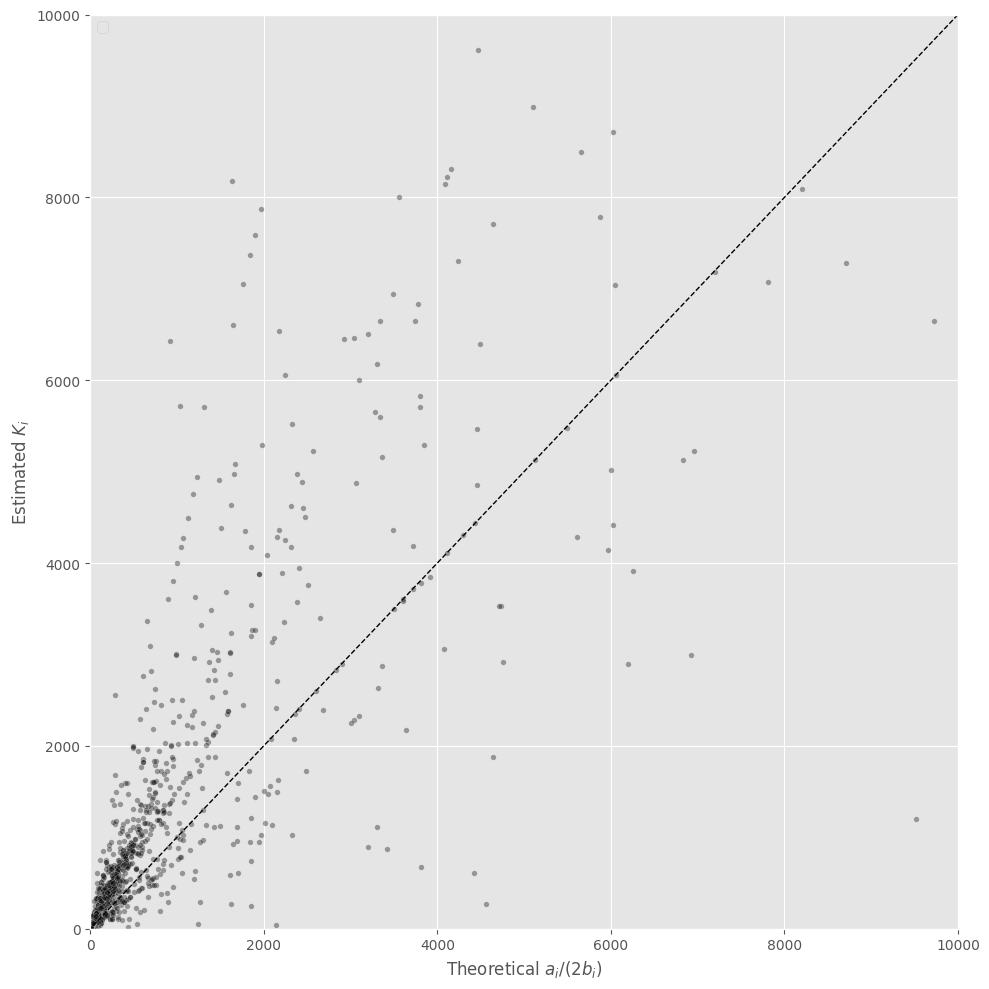
\includegraphics[width=0.45\textwidth]{K_K_theory_10000.png}
    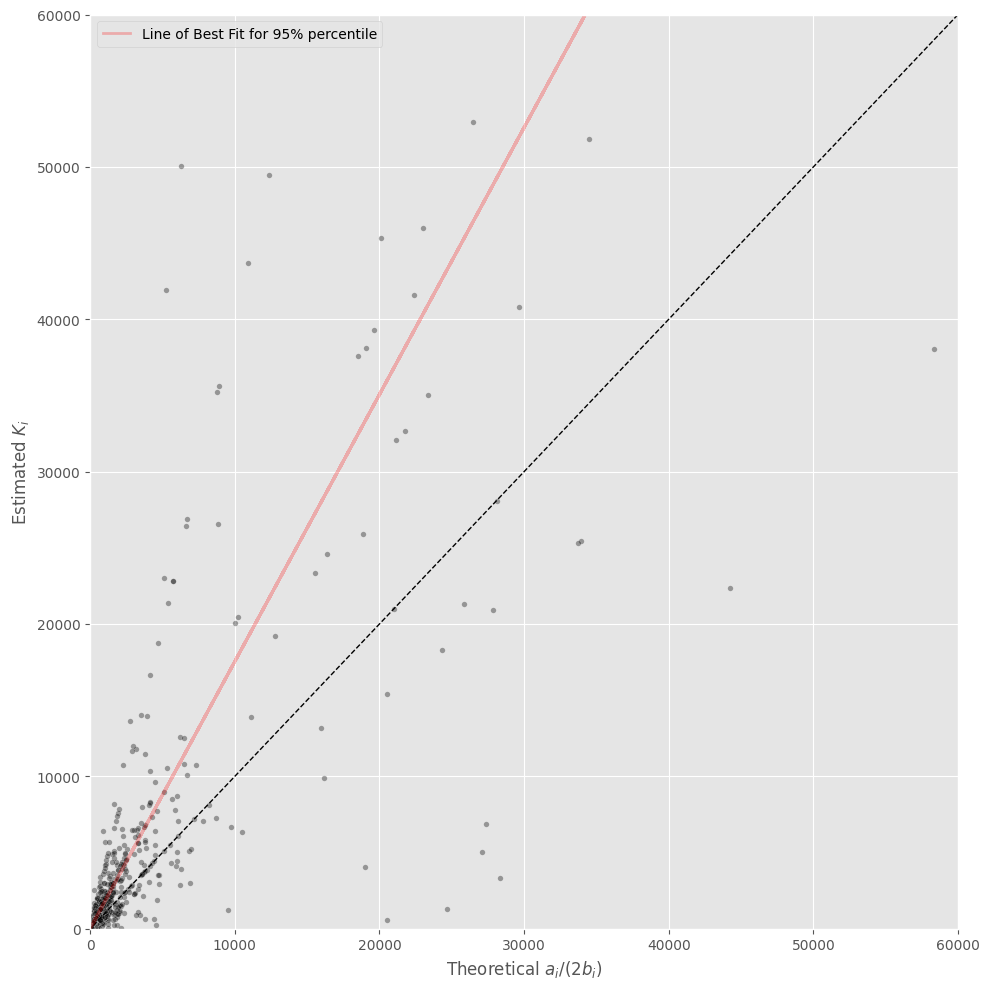
\includegraphics[width=0.45\textwidth]{K_K_theory_60000_bestfit95.png}
    \caption{Left: Scatter plot with theoretical active management limit against estimated active management break point. Right: Zoomed out scatter with 95\% percentile subset line of best fit.}
    \label{fig:combined-scatter}
\end{figure}

Regressing $K_i = c\  + dK_i^{theory}\ + \nu_i$ shows a significant $K_i\simeq1.75·K_i^{theory}$ for the 95\% percentile and still significant $1.46$ times for the 99\%, backing the result that funds tend to over-manage. The next logical step is comparing how these estimates relate to the actual fund sizes.

\par
As the non linear model nests the linear specification, it could potentially handle the case where a manager is able to invest any amount of funds actively and successfully add value, resulting in an estimated $K_i$ greater than the fund historical sizes, or the case where the fund is a structure that basically indexes all of the inflows characterized by significantly $K_i$ smaller than its size. 

\par
Instead of by percentiles of theoretical K, now we classify the funds by their average size over time and present a similar table for the 10 deciles of sizes.

\begin{table}[H]
    \centering
    \caption{Summary of Estimates by Fund Size Decile}
    \label{tab:decile-estimates-new-3}
    \begin{tabular}{lrrrrrr}
        \hline
        Decile & K avg & K theory avg & K diff & mean size & Funds Inc & $K>K$ theory \\
        \hline
        1 & 68.51 & 37.19 & 31.32 & 33.62 & 141 & 127 \\
        2 & 204.53 & 145.14 & 59.39 & 58.58 & 140 & 116 \\
        3 & 245.59 & 130.52 & 115.07 & 90.79 & 141 & 124 \\
        4 & 333.60 & 202.53 & 131.07 & 130.53 & 140 & 119 \\
        5 & 1406.79 & 826.83 & 579.96 & 200.18 & 141 & 122 \\
        6 & 1410.88 & 1223.27 & 187.61 & 282.06 & 140 & 108 \\
        7 & 1390.45 & 923.27 & 467.18 & 435.28 & 140 & 116 \\
        8 & 2652.42 & 1446.91 & 1205.52 & 692.60 & 141 & 120 \\
        9 & 5012.30 & 3412.33 & 1599.97 & 1184.42 & 140 & 105 \\
        10 & 10856.63 & 8349.82 & 2506.81 & 4703.38 & 141 & 100 \\
        \hline
    \end{tabular}
\end{table}
The same dynamic is still present per deciles: a big portion of each decile are funds where estimated $K_i$ is bigger than the theoretical but the top deciles of average biggest funds over time see on average the trend reversed because these cohorts contain the parasitic cases where $K^{theory}_i$ becomes orders of magnitude bigger than the normal range of values of the fund.
One could hypothesize that the reason this is happening is because the bigger funds are probably close in principle to indexing and are estimated to have such a low cost relative to their size, that the estimated small $b_i$ makes $K^{theory}_i$ big while in reality the fund is actually just indexing a majority of the funds and the optimization isn't able to escape the local minima it found in the first place. 

\par As mentioned in section 2.1, the dataset has some of the funds classified by style depending on their capitalization, turnover and commercial channel. From the 1405 funds in the main analysis, 916 have classification. 

\begin{table}[H]
    \centering
    \caption{Summary of Estimates by Fund Style}
    \label{tab:style-estimates}
    \begin{tabular}{lrrrrr}
        \hline
        Style & K avg & K theory avg & K diff & Funds Inc & $K>K$ theory \\
        \hline
        1 & 1061.14 & 748.44 & 312.70 & 25 & 16 \\
        2 & 2025.84 & 1094.22 & 931.61 & 57 & 46 \\
        3 & 1349.85 & 1591.19 & -241.34 & 53 & 44 \\
        4 & 2259.05 & 2025.29 & 233.76 & 43 & 29 \\
        5 & 497.87 & 277.67 & 220.19 & 40 & 36 \\
        6 & 1588.46 & 817.18 & 771.28 & 46 & 43 \\
        7 & 2724.70 & 1708.08 & 1016.63 & 31 & 26 \\
        8 & 1145.22 & 493.86 & 651.36 & 36 & 28 \\
        9 & 2352.64 & 1300.96 & 1051.69 & 53 & 45 \\
        10 & 3396.51 & 3418.43 & -21.92 & 29 & 22 \\
        11 & 2213.19 & 1470.13 & 743.06 & 29 & 26 \\
        12 & 1349.32 & 869.68 & 479.63 & 45 & 39 \\
        13 & 3792.85 & 2959.53 & 833.31 & 79 & 62 \\
        14 & 2901.33 & 2460.40 & 440.93 & 101 & 86 \\
        15 & 2412.00 & 1364.85 & 1047.15 & 78 & 72 \\
        16 & 2799.91 & 1926.41 & 873.50 & 75 & 58 \\
        17 & 3418.13 & 2200.99 & 1217.14 & 49 & 34 \\
        18 & 3581.00 & 2570.86 & 1010.14 & 47 & 42 \\
        \hline
    \end{tabular}
\end{table}

As argued earlier, theoretically there is no population of funds in mathematical terms where the parameters of the funds are drawn from a distribution. That is the reason we have not modeled bundles of funds or portfolios. However, it could be that styles, because of underlying market exogenous factors did affect the behavior of the fund in a noticeable way but from table \ref{tab:style-estimates} there is no single trait which dramatically affects the results. Larger capitalization funds, 13 to 18 styles, have larger differences as we have already seen in previous tables. The only notable exception is style three which corresponds to small-cap, high-turnover broker-sold funds but it is difficult to draw a conclusion when other small caps do not present this behavior and nor do other high turnover or broker-sold styles. If we take a look at the estimation for the faulty funds within style 3 in table \ref{tab:style3-neg-k-diff}
\begin{table}[H]
    \centering
    \caption{Estimates for Style 3 Funds with Negative K difference}
    \label{tab:style3-neg-k-diff}
    \begin{tabular}{lrrrrrr}
        \hline
        fund\_id & a & b & TNA\_median & K & K\_theory & K\_difference \\
        \hline
        100763 & 0.007819 & 1.14e-06 & 169.57 & 870.76 & 3422.69 & -2551.93 \\
        102417 & 0.012718 & 1.83e-05 & 900.30 & 346.61 & 347.06 & -0.45 \\
        103299 & 0.005783 & 1.41e-07 & 211.05 & 574.73 & 20511.38 & -19936.65 \\
        105269 & 0.003335 & 2.44e-07 & 91.10 & 5125.15 & 6827.84 & -1702.69 \\
        105458 & 0.002566 & 5.27e-08 & 415.28 & 18267.61 & 24336.54 & -6068.92 \\
        106101 & 0.010531 & 3.07e-04 & 24.40 & 17.12 & 17.14 & -0.02 \\
        106485 & 0.007304 & 2.58e-05 & 89.57 & 96.42 & 141.63 & -45.21 \\
        400127 & 0.001901 & 5.12e-07 & 485.50 & 1209.93 & 1854.71 & -644.78 \\
        410447 & 0.008020 & 6.17e-05 & 117.26 & 63.51 & 65.00 & -1.49 \\
        \hline
    \end{tabular}
\end{table}

we discover that theoretical $a_i/2b_i$ is completely outside the range of sizes that most of these funds have ever been. This will lead us naturally into the next section because for this funds $a$ and $b$ have to be very similar for both models since the range of sizes is completely contained inside the domain of the linear piece of the model. 

\par
Before continuing to the comparison, we need to check how often is $K_i$ falling outside the range of sizes. Theoretically these would be funds completely modeled by the linear specification.

\begin{table}[h!]
    \centering
    \caption{Summary of Estimates by Fund Size Decile}
    \label{tab:decile-funds-maxTNA}
    \begin{tabular}{lrrrrr}
        \hline
        Decile & K avg & K theory avg & Funds Inc &  $K>K$ theory & $K< max_t(q_{i,t})$ \\
        \hline
        1 & 68.51 & 37.19 & 141 & 127 & 110 \\
        2 & 204.53 & 145.14 & 140 & 116 & 105 \\
        3 & 245.59 & 130.52 & 141 & 124 & 98 \\
        4 & 333.60 & 202.53 & 140 & 119 & 106 \\
        5 & 1406.79 & 826.83 & 141 & 122 & 99 \\
        6 & 1410.88 & 1223.27 & 140 & 108 & 101 \\
        7 & 1390.45 & 923.27 & 140 & 116 & 106 \\
        8 & 2652.42 & 1446.91 & 141 & 120 & 110 \\
        9 & 5012.30 & 3412.33 & 140 & 105 & 112 \\
        10 & 10856.63 & 8349.82 & 141 & 100 & 111 \\
        \hline
    \end{tabular}
\end{table}

The last column in table \ref{tab:decile-funds-maxTNA} reveals that basically $25\%$ of the funds are being estimated to not have any non -linear kink in their gross alpha.


\subsection{Gross alpha: a and b estimates}
Evaluating the fit of the model requires analyzing the gross alpha and asses if the slight improvement in the fit keeps the alpha relatively in expected ranges.


With these tables it can be tempting to check if 
$$
\frac{a_{avg}}{b_{avg}}=K^{theory}_{avg}
$$

but due to Jensen's inequality (check appendix \ref{app:jensen}), we can not simply pull the values from the table to build an average model as

$$ \frac{1}{N} \sum_{i=1}^{N} \left( \frac{a_i}{2b_i} \right) \neq \frac{\left( \frac{1}{N} \sum a_i \right)}{\left( 2\frac{1}{N} \sum b_i \right)} $$

so the averages in the column of $K_{theory}$ do not correspond to a model estimated to have that row's average $a$ and $b$.

\par First we have to check how $a_i$ and $b_i$ behave for the funds mentioned at the end of the previous section, those that are being approximated with the linear model that is nested in the full model.

\begin{table}[H]
    \centering
    \caption{Funds where $K>max_t(q_{i,t})$}
    \label{k>max-alin-bln-a-b}
    \begin{tabular}{lrrrrrrrr}
        \hline
        D & a lin avg & a avg & b lin avg & b avg & $K^{theory}_{avg}$  & $max(size)^{avg}$ & Inc & $K>K_{the}$ \\
        \hline
        1 & 0.005717 & 0.005717 & 6.75e-05 & 6.75e-05 & 113.85 & 80.23 & 31 & 26 \\
        2 & 0.004145 & 0.004145 & 1.88e-05 & 1.88e-05 & 444.61 & 170.83 & 35 & 23 \\
        3 & 0.006704 & 0.006704 & 2.64e-05 & 2.64e-05 & 278.99 & 272.85 & 43 & 39 \\
        4 & 0.006491 & 0.006491 & 1.52e-05 & 1.52e-05 & 500.05 & 403.16 & 34 & 28 \\
        5 & 0.005536 & 0.005536 & 6.84e-06 & 6.84e-06 & 2276.84 & 680.94 & 42 & 35 \\
        6 & 0.005671 & 0.005671 & 4.44e-06 & 4.44e-06 & 2903.90 & 959.01 & 39 & 29 \\
        7 & 0.005390 & 0.005390 & 2.68e-06 & 2.68e-06 & 2541.39 & 1772.87 & 34 & 28 \\
        8 & 0.004646 & 0.004646 & 1.57e-06 & 1.57e-06 & 4144.17 & 2730.34 & 31 & 30 \\
        9 & 0.005363 & 0.005363 & 9.98e-07 & 9.98e-07 & 11793.00 & 5195.37 & 28 & 26 \\
        10 & 0.006490 & 0.006490 & 4.99e-07 & 4.99e-07 & 12457.51 & 16456.65 & 30 & 27 \\
        \hline
    \end{tabular}
\end{table}

For every decile, it is indeed found that for the subset of funds left in each of them, the models are identical. For the cohort of biggest funds there are some irregularities that skew the averages because the funds of this decile have the biggest ranges in sizes. For the rest, the funds are not only smaller than $K_i$ but also smaller on average than their theoretical optimal size $K_i^{theory}=q_i^*=a_i/2b_i$. The estimated $K$ is meaningless for them. These would be funds actively managing a suboptimal amount of funds but still managing all of the money from all of their investors, so they would be struggling to raise enough funds to extract all the value they theoretically could.
\par As we can see in table \ref{tab:decile-estimates-final-pvals} while the results are not necessarily significant on average, some things stand out. The average fully actively managed funds range between 0.4\% and 0.65\% first dollar alphas. With 1000 million worth of assets under management, a fund would be bringing in between around 5.7 million in revenue and spending around 4.4 million to do it. The most interesting thing is that while $a$ remains within the same order magnitude, average $b$ decreases exactly the inverse amount that size increases moving from $7\times10^{-5}$ for funds that have managed less than a 100 million to $5\times10^{-7}$ for funds in the tens of billions. This is the slope of the model and with symmetrically distributed small gross alphas plus big fund sizes, we expect them to be this small. This is a very good reminder than funds have mostly fixed fees, stable $a$ across cohorts, to stay competitive in the market and have to compensate for diseconomies of scale to stay in business. This will first make them adopt lower operating cost structures to manage more money before increasing their fees to earn more. In doing so, these funds would be pushing further from their theoretical optimal volume of actively managed money. This is actually in line with the main findings: these funds are chasing managing more funds rather than optimizing value generation with their smaller size, higher costs structure. 

\par
With the models being identical we can use the linear model to asses the significance of the coefficients. In the following table we list the average coefficients in each decile as well as it average standard deviation. Cost coefficient $b$ presents high average standard deviation among the funds in every decile and is rarely found to be significantly different than zero. The highest significance is found for the biggest funds where the coefficient is found to have an average p-value of 0.1412.



\begin{table}[h!]
    \centering
    \caption{Exploratory analysis for funds where $K>max_t(q_{i,t})$}
    \label{tab:decile-estimates-final-pvals}
    \begin{tabular}{llrrrr}
        \toprule
        Decile & a lin/no lin avg & a standard dev avg & b lin/no lin avg & b standard dev avg \\
        \midrule
        1 & 0.005717 & 0.003364 & 6.75e-05 & 9.30e-05 \\
        2 & 0.004145 & 0.002489 & 1.88e-05 & 2.75e-05 \\
        3 & 0.006704* & 0.003743 & 2.64e-05 & 4.29e-05 \\
        4 & 0.006491 & 0.003959 & 1.52e-05 & 2.02e-05 \\
        5 & 0.005536 & 0.003060 & 6.84e-06 & 8.41e-06 \\
        6 & 0.005671* & 0.003238 & 4.44e-06 & 5.45e-06\\
        7 & 0.005390** & 0.002224 & 2.68e-06 & 2.04e-06 \\
        8 & 0.004646** & 0.001741 & 1.57e-06 & 1.22e-06 \\
        9 & 0.005363** & 0.002174 & 9.98e-07 & 9.66e-07 \\
        10 & 0.006490*** & 0.002567 & 4.99e-07 & 4.91e-07 \\
        \bottomrule
        \multicolumn{6}{l}{\footnotesize * significant at 10\%; ** at 5\%; *** at 1\% based on the \textbf{average p-values} from the fund regressions.}
    \end{tabular}
\end{table}

The first dollar alpha coefficient $a$ on the other hand is on average significant, particularly for the bigger cohorts. For the tenth decile, the average p value is lower than 0.01.


\par
The relevant question now is how do these previous observations compare to the funds where $K_i>max_t(q_{i,t})$, that is, the funds for which the gross alpha actually presents a kink that could explain a switch in their investment strategy.

\begin{table}[H]
    \centering
    \caption{Funds where $K<max_t(q_{i,t})$}
    \label{tab:estimates-deciles-k<max1}
    \begin{tabular}{lrrrrr}
        \toprule
        Dec & $K$ avg & $K_{theory}$ avg & max(size) avg & Funds Inc & $K>K_{theory}$ \\
        \midrule
        1 & 27.81 & 15.58 & 78.92 & 110 & 101 \\
        2 & 59.99 & 45.32 & 176.86 & 105 & 93 \\
        3 & 92.56 & 65.38 & 293.90 & 98 & 85 \\
        4 & 162.54 & 107.10 & 462.60 & 106 & 91 \\
        5 & 243.90 & 211.67 & 711.52 & 99 & 87 \\
        6 & 404.76 & 574.31 & 1135.26 & 101 & 79 \\
        7 & 541.02 & 404.26 & 1691.21 & 106 & 88 \\
        8 & 874.74 & 686.77 & 2497.29 & 110 & 90 \\
        9 & 1654.16 & 1317.17 & 5101.61 & 112 & 79 \\
        10 & 6209.64 & 7239.64 & 20200.89 & 111 & 73 \\
        \bottomrule
    \end{tabular}
\end{table}


As expected, for this subset of funds the theoretical size threshold is below the sizes of the funds and as seen previously in section 3.1, even after removing the funds that are essentially linear, the estimated position of the switch between the linear and non-linear pieces is greater than $K_{theory}$ for most of the funds. The only exception in table \ref{tab:estimates-deciles-k<max1} with respect to table \ref{tab:decile-estimates-new-3} is the subset of funds from the sixth decile that now presents on average bigger theoretical $K$. Average sizes also grow similarly to average $K$ over the deciles. 


\par In comparison to the fully linear funds, table \ref{tab:estimates-deciles-k<max2} displays greater average first dollar alpha $a$ in the linear specification than before but still similar across deciles. The big changes are in the coefficient provided by the nonlinear model which are for every decile much higher with greater discrepancies between them. With $b$ there is a similar situation, with bigger funds having lower management costs but not in the same consistent fashion as before.


\begin{table}[H]
    \centering
    \caption{Funds where $K<max_t(q_{i,t})$}
    \label{tab:estimates-deciles-k<max2}
    \begin{tabular}{lrrrr}
        \toprule
        Decile & $a^{lin}$ avg & $a$ avg & $b^{lin}$ avg & $b$ avg \\
        \midrule
        1 & 0.009074 & 0.290702 & 2.01e-04 & 0.040090 \\
        2 & 0.007770 & 0.271527 & 7.47e-05 & 0.039647 \\
        3 & 0.007067 & 0.022995 & 3.82e-05 & 0.003093 \\
        4 & 0.007568 & 0.457151 & 2.79e-05 & 2.261319 \\
        5 & 0.006923 & 2.414604 & 1.59e-05 & 0.020323 \\
        6 & 0.007227 & 0.018576 & 1.10e-05 & 0.000109 \\
        7 & 0.007197 & 0.284495 & 7.06e-06 & 0.002311 \\
        8 & 0.007126 & 0.124551 & 4.36e-06 & 0.001442 \\
        9 & 0.007285 & 0.015050 & 2.18e-06 & 0.000032 \\
        10 & 0.007160 & 13.588227 & 7.55e-07 & 0.009482 \\
        \bottomrule
    \end{tabular}
\end{table}

We have included this tables to illustrate how under this model with unbounded estimation, very few cases have a great influence on the study. After an analysis per decile we find that just a handful of spurious estimations are polluting the entire table. 
\par By removing cases where $a,b>1$ which would already be unbelievably high values for any of them, we get the following corrected tables with minimal reduction in the number of funds. This is much clearer picture of how under the non-linear specification the average first dollar alpha $a$ is found to decrease as funds increase in size, with costs coefficient $b$ decreasing again inversely. In both cases the coefficients are bigger than in the linear case, even without the flawed funds that were still present in table \ref{tab:estimates-deciles-k<max2}.
            

\begin{landscape}
    \begin{table}[h!]
        \centering
        \begin{threeparttable}
            \caption{\Large Clean Sample of Funds where $K<max_t(q_{i,t})$}
            \label{tab:estimates-deciles-combined-k<max}
            \begin{tabular}{lrrrrrrrrrr}
                \toprule
                D & a lin avg & a avg & b lin avg & b avg & K avg & K theory avg & Max size avg & Mean size & Funds Inc & $K>K$ theory \\
                \midrule
                1 & 0.008923 & 0.047571 & 1.89e-04 & 0.011030 & 28.63 & 16.07 & 80.68 & 33.32 & 105 & 96 \\
                \addlinespace
                2 & 0.007925 & 0.034179 & 7.52e-05 & 0.003215 & 61.74 & 46.80 & 176.91 & 58.41 & 101 & 89 \\
                \addlinespace
                3 & 0.007067 & 0.022995 & 3.82e-05 & 0.003093 & 92.56 & 65.38 & 293.90 & 89.65 & 98 & 85 \\
                \addlinespace
                4 & 0.007625 & 0.015394 & 2.78e-05 & 0.000173 & 165.66 & 109.16 & 465.23 & 127.04 & 104 & 89 \\
                \addlinespace
                5 & 0.007010 & 0.014662 & 1.60e-05 & 0.000121 & 246.47 & 214.81 & 719.27 & 198.93 & 97 & 85 \\
                \addlinespace
                6 & 0.007227 & 0.018576 & 1.10e-05 & 0.000109 & 404.76 & 574.31 & 1135.26 & 276.04 & 101 & 79 \\
                \addlinespace
                7 & 0.007221 & 0.021596 & 7.03e-06 & 0.001143 & 544.05 & 407.04 & 1701.84 & 439.92 & 105 & 87 \\
                \addlinespace
                8 & 0.007145 & 0.013491 & 4.34e-06 & 0.000028 & 885.70 & 696.87 & 2511.60 & 697.55 & 108 & 88 \\
                \addlinespace
                9 & 0.007285 & 0.015050 & 2.18e-06 & 0.000032 & 1654.16 & 1317.17 & 5101.61 & 1187.82 & 112 & 79 \\
                \addlinespace
                10 & 0.007057 & 0.013084 & 7.05e-07 & 0.000007 & 6274.22 & 7347.80 & 20442.47 & 4646.68 & 109 & 71 \\
                \addlinespace
                \bottomrule
            \end{tabular}
            \begin{tablenotes}
                \item[]
            \end{tablenotes}
        \end{threeparttable}
    \end{table}
\end{landscape}


 In a representative cohort with similar amount of around a thousand million under management median size, we can find great diversity pointing once again at the theoretical flexibility to fix fees and have different returns. There can be funds with $a_i$ as high $3.5\% $ and high management cost, considerably higher than those found by the linear specification, that very quickly reach their limit of optimal active management and then seem to be indexing. The model is promising as it captures very early dynamics where the fund manages to find a slight return edge that is very quickly dissipated with growth. 


\begin{figure}[H]
    \centering
    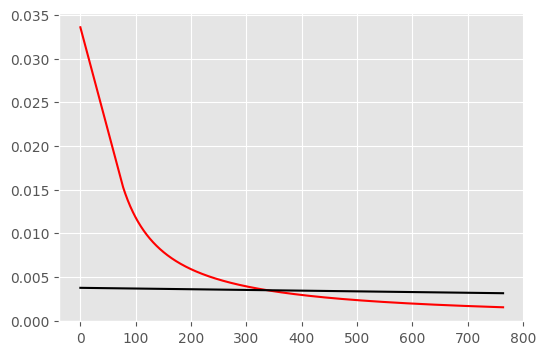
\includegraphics[width=0.43\textwidth]{Fund101112.png}
    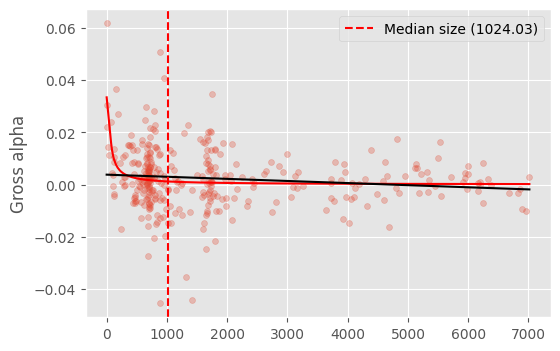
\includegraphics[width=0.55\textwidth]{Fund101112_scatter.png}
    \caption{Left: Linear and non linear models for one of these aforementioned funds. Right: Graphs of the 2 models with the scattered points}
    \label{fig:fund101112}
\end{figure}

In this particular case, the fund presents higher returns over the benchmark factors at sizes below a 100 million that decline fast with size or at least are matched with lower than benchmark returns so the linear piece fits the early stages while the gross alpha decreases to almost zero as the fund indexes. This is perfectly consistent with a fund doing small-cap deals and indexing all of the excess funds. In this example, the manager is bringing around 2.5 million net, fundamentally coming from the active management of around 75 million since the excess is assumed to have a negligible cost and as seen in figure \ref{fig:fund101112} with very symmetrically distributed returns, as it is expects in the broad market. Under the linear specification, the fund has to be managing 825 million to extract the same value and there is no longer a way to model different investment strategies taking place inside the same fund.

\par
A better manager will be characterized then not by his gross returns, that can be lower like the following fund from figure \ref{fig:fund109823} which earns a lower $2.7\%$, or the absolute size of the fund, which is again of median size around 1000 million, but by the value-added.


\begin{figure}[H]
    \centering
    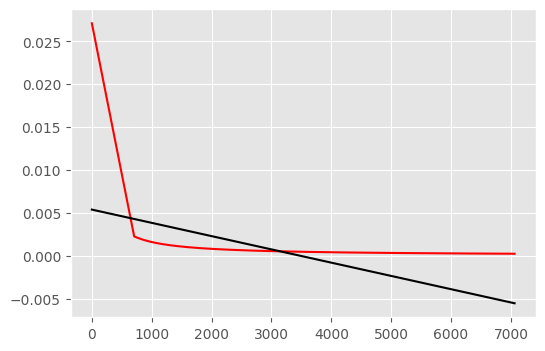
\includegraphics[width=0.43\textwidth]{Fund109283.png}
    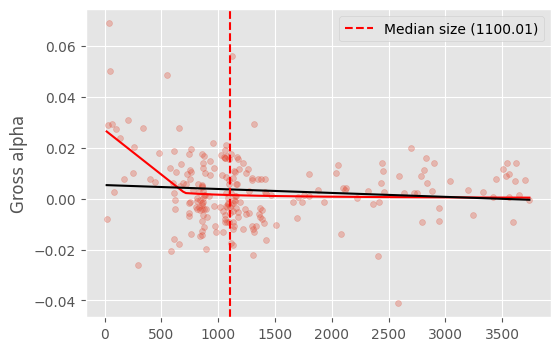
\includegraphics[width=0.55\textwidth]{Fund109283_scatter.png}
    \caption{Left: Linear and non linear models for one of these aforementioned funds. Right: Graphs of the 2 models with the scattered points}
    \label{fig:fund109823}
\end{figure}

With lower returns, lower costs and actively managing 700 million, the fund in figure \ref{fig:fund109823} is expected to generate less profit at 1.59 million. But we cannot forget what we showed in the first empirical results: managers tend to over-manage and if this fund started indexing much earlier, around the optimal theoretical 385 million, with less active management, profit could climb up to 5.22 million. 


\par
In any case, for most funds the higher $a$ found by the non-linear model are a bit closer to what we would expect to find the market with close to $5\% $ return for smaller funds, down to $1.5\%$ for the bigger size cohorts, while the linear specification has to fit the entire size history returning first dollar alphas that are on the lowest part of the spectrum for an actively managed fund, lower than $0.8\%$, and too big for a totally passively managed fund. This suggests some advantage in the non-linear model to explain reality.


\par Having filtered the funds that are not modeled better by the piece-wise model, one notable result is how the average $a$ decreases to be just a bit bigger that the usual fees of the funds, found to be on average lower than $1.3\% $ for basically any fund. Size erases most active management opportunities and returns of the fund are likely just coming from management fees.

\par Before moving on we must address what is obvious when looking at figures \ref{fig:fund101112} and \ref{fig:fund109823}. While the non-linear model has increased capabilities to capture funds dynamics over the base, gross alpha is very difficult to capture with such a simple model. The scatter plots represent estimated gross alphas that none of models can come close to properly model, especially as the fund sizes increase and the returns perform more under the usual stylized facts as seen in figures \ref{fig:fund101112} and \ref{fig:fund109823}. Gross alphas are not observed and have to be derived from the returns of the funds as explained at the end of section 2.3 and after correcting for the benchmark factors they have similar distributions to them. 


\begin{figure}[H]
    \centering
    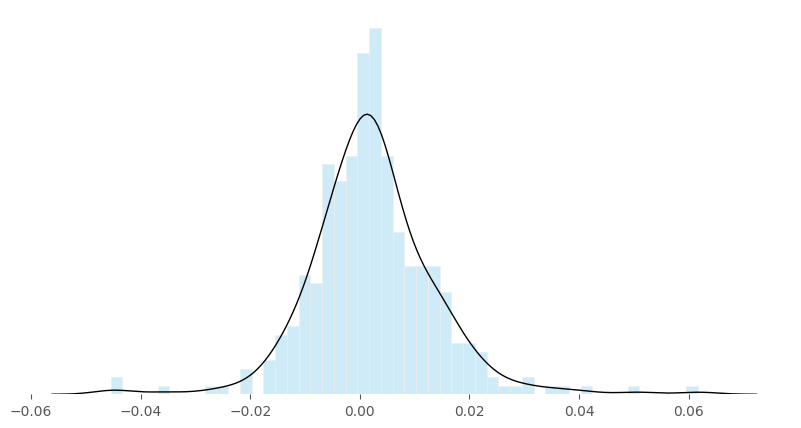
\includegraphics[width=0.80\textwidth]{HistogramFatTails101112.png}
    \includegraphics[width=0.80\textwidth]{Fund101557_HistogramFatTails.png}
    \caption{The two extremes of the gross alpha distribution ranging from very symmetric returns (up) to the more representative positively skewed (down) with fatter tails.}
    \label{fig:fund101112_grossalpha}
\end{figure}

\par In the following table \ref{tab:combined-moments} we report the moment averages of the gross the alphas per decile, similar to the distribution for an equally weighted portfolio of funds per decile. Contrary to the negative skewness with e a thicker left tail commonly found for returns, gross alphas under the non-linear model are on average very small, positively skewed but positive, $0.3\%$ excess over benchmarks with consistent standard deviation across all the deciles. The distribution presents on average fat tails with high kurtosis for every cohort in every subset. For the big funds in the tenth decile there is a considerable reduction in skewness driven by the big linear funds $K>max_{t}(q_{i,t})$ very low skewness.

\begin{table}[h!]
    \centering
    \begin{threeparttable}
        \caption{Average Moments of the Gross Alpha}
        \label{tab:combined-moments}
        \begin{tabular}{lrrrrrr}
            \toprule
            \multicolumn{7}{c}{\textbf{Population Averages}} \\
            \midrule
            \multicolumn{1}{c}{} & Funds Inc & Mean Size & Mean & Std. Deviation & Skewness & Kurtosis \\
            \midrule
            & 1405 & 782.44 & 0.003447 & 0.017053 & 0.135969 & 2.596025 \\
            \midrule
            \multicolumn{7}{c}{\textbf{Average Moments by Decile}} \\
            \midrule
            D & Funds Inc & Mean Size & Mean & Std. Deviation & Skewness & Kurtosis \\
            \midrule
            \multicolumn{7}{c}{\textit{Entire Population}} \\
            \midrule
            1 & 141 & 33.62 & 0.002765 & 0.017426 & 0.100555 & 1.876853 \\
            2 & 140 & 58.58 & 0.002920 & 0.017507 & 0.128062 & 2.732960 \\
            3 & 141 & 90.79 & 0.003331 & 0.017922 & 0.031154 & 2.520256 \\
            7 & 140 & 435.28 & 0.003483 & 0.016109 & 0.194121 & 2.223731 \\
            8 & 141 & 692.60 & 0.003449 & 0.015947 & 0.221892 & 3.002236 \\
            9 & 140 & 1184.42 & 0.003991 & 0.017536 & 0.252956 & 2.936116 \\
            10 & 141 & 4703.38 & 0.004245 & 0.015850 & 0.087611 & 2.723865 \\
            \midrule
            \multicolumn{7}{c}{\textit{$K > \text{max}$ Size}} \\
            \midrule
            1 & 31 & 35.92 & 0.003248 & 0.014276 & 0.131568 & 2.309949 \\
            2 & 35 & 59.44 & 0.002956 & 0.014720 & -0.000222 & 5.306359 \\
            3 & 43 & 93.38 & 0.003975 & 0.017988 & -0.173592 & 3.690773 \\
            7 & 34 & 420.38 & 0.003895 & 0.014387 & 0.042726 & 1.885665 \\
            8 & 31 & 670.21 & 0.003316 & 0.013188 & 0.048453 & 1.886658 \\
            9 & 28 & 1170.84 & 0.003884 & 0.015525 & 0.235531 & 3.893577 \\
            10 & 30 & 4848.19 & 0.004442 & 0.013539 & 0.000060 & 2.192981 \\
            \midrule
            \multicolumn{7}{c}{\textit{K$<$ max Size}} \\
            \midrule
            1 & 105 & 33.32 & 0.002701 & 0.018337 & 0.079514 & 1.789763 \\
            2 & 101 & 58.41 & 0.003048 & 0.018404 & 0.176880 & 1.934706 \\
            3 & 98 & 89.65 & 0.003048 & 0.017893 & 0.120992 & 2.006662 \\
            4 & 104 & 127.04 & 0.003206 & 0.017979 & 0.227941 & 1.975858 \\
            5 & 97 & 198.93 & 0.003234 & 0.018536 & 0.229874 & 2.716246 \\
            6 & 101 & 276.04 & 0.003338 & 0.017600 & -0.012527 & 4.087290 \\
            7 & 105 & 439.92 & 0.003384 & 0.016753 & 0.242192 & 2.356260 \\
            8 & 108 & 697.55 & 0.003520 & 0.016811 & 0.284897 & 3.353093 \\
            9 & 112 & 1187.82 & 0.004018 & 0.018039 & 0.257312 & 2.696751 \\
            10 & 109 & 4646.68 & 0.004276 & 0.016606 & 0.113336 & 2.910375 \\
            \bottomrule
            \bottomrule
        \end{tabular}
    \end{threeparttable}
\end{table}


As a consequence, the coefficient of determination after subtracting the benchmark from the returns (to retrieve the gross alpha) is low. Even if the fit is better for the small sizes, the model cannot capture the full range of symmetric alphas present across the greater sizes because the gross alphas are too spread. For the subset of 1405 funds, the linear model average $R^2_{lin}$ is $0.023$ that climbs to $0.036$ average for the non-linear model. If the computation is restricted to funds that present a kink where it can have an effect, when $K_i<max_t(q_{i,t})$, it improves marginally to an average $0.044$. The $R^2$ of the gross returns increases from around 0.88 to 0.94 between the linear and non-linear specifications.


\par
One question remains to answer and that is if under this non-linear model specification and with a tendency to manage more money than it is optimal, the managers are actually extracting value-added. 


\section{Value creation: value-added}

By design, for a fund where the kink is estimated to be inside its range of sizes, we are expecting the non-linear specifications to fit the funds as it should allow two mechanisms:

\begin{itemize}
    \item The first is used by funds with very high returns at small sizes that under this specification can have a steeper linear piece until the estimated breaking point while the fully linear specification slope tends to be much flatter to fit the big size symmetrical returns. This is characterized by $b^{noLin}_i>b_i^{lin}$. Gross alpha for this funds is very high in the beginning but decreases fast.
    \item The second happens for funds where $b^{noLin}_i<b_i^{lin}$. The linear piece is flatter.
\end{itemize}

From the funds left in table \ref{tab:estimates-deciles-combined-k<max}, 977 fall into the first category and 81 into the second, proving further that diseconomies of scale are present in the sector. The reason we mention this is because ultimately we are interested in value-added, which is defined as $V_{i,t}=TR_{i,t}-TC_{i,t}$ but from \ref{grosslin}, \ref{grossnolin} and \ref{model} it is trivial to see that 

\begin{equation}
    V_{i,t}=TR_{i,t}-TC_{i,t}=q_{i,t}\alpha_{i,t}.
\end{equation}

So we expect value added to be very explosive for funds in the first category, funds that have to make most of the profit from managing a small portion of their funds and less so for the second. In any case, for both subgroups, under both specification, managers must strive to bring in enough funds to reach their optimal operating point $q_{i,t}^*$ and going over it does not have any downsides as long as they index but for the funds found previously to be very lineal yet still having $K<max_{t}(q_{i,t})$, the opposite is true as they can potentially destroy value instead of creating it.

\par To analyze this we present very similar tables as before but now we start by reporting the average value-added produced by the funds. Value-added $V_{i,t}$ has two subscripts because each fund $i$ produces a certain amount of value-added per period (month in our case) so we first average over time and then over the bundle of funds from a decile or a subgroup. As always, it is necessary to ignore some extreme cases.



\begin{table}[H]
    \centering
        \caption{Average Value Added $K > \text{max}$ Size}
        \label{tab:value-added-size-k>max}
        \begin{tabular}{lrrrrrrrrrr}
            \toprule
            \multicolumn{1}{c}{Metric} & \multicolumn{10}{c}{Decile} \\
            \cmidrule(lr){2-11}
            \multicolumn{1}{c}{} & 1 & 2 & 3 & 4 & 5 & 6 & 7 & 8 & 9 & 10 \\
            \midrule
            Avg. Val Added & 0.1 & 0.2 & 0.3 & 0.5 & 0.8 & 1.2 & 1.6 & 2.1 & 4.6 & 19.3 \\
            Avg.Med Size & 35.9 & 59.4 & 93.4 & 139.1 & 200.4 & 297.7 & 420.4 & 670.2 & 1170.8 & 4848.2 \\
            \bottomrule
        \end{tabular}
\end{table}


Since $K_i > max_{t}(q_{i,t})$ these funds are theoretically never even reaching their maximum active management size and it is almost a situation of chasing the threshold away, value-added for every decile is between $0.3\% $ and $0.4\% $ of the average median volume of assets under management.

\begin{figure}[h!]
    \centering
    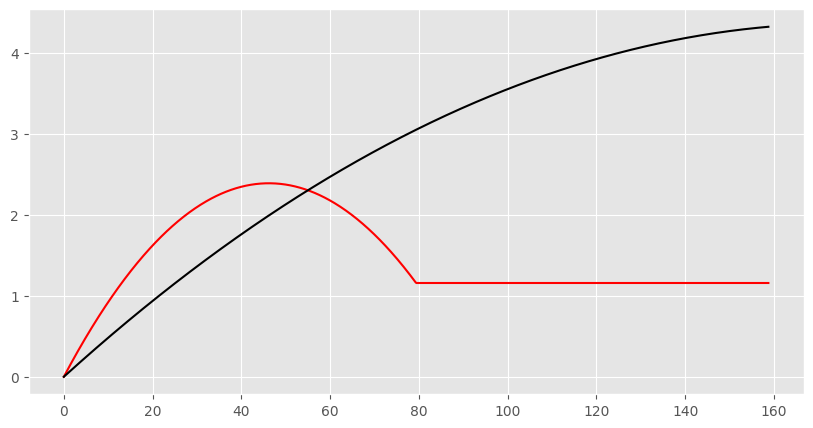
\includegraphics[width=0.45\textwidth]{ChasingOptimal.png}
    \caption{Value added model for a fund computed under the linear specification (black) and the non-linear model (red)}
    \label{fig:ChasingOptimal}
\end{figure}

In figure \ref{fig:ChasingOptimal} we show the 2 models for the same fund to illustrate how under the linear model, the theoretical maximizing size can be so big that it is unfeasible to reach, but for a non-linear fund it is rather easy not only to reach it but to over-manage instead of indexing earlier. This fund was not chosen randomly, it is one of the funds with the best fit from the dataset and the highest small-size gross alpha, potentially a fund that could greatly benefit from indexing sooner to preserve those early returns. This is obviously easier said than done, as this fund is indexing at 80 million with respect to the theoretical 46 while having a median volume under management of 175 million.


\begin{table}[H]
    \centering
    \begin{threeparttable}
        \caption{Average Val Add $K < \text{max}$ Size}
        \label{tab:value-added-size-k<max}
        \begin{tabular}{lrrrrrrrrrr}
            \toprule
            \multicolumn{1}{c}{Metric} & \multicolumn{10}{c}{Decile} \\
            \cmidrule(lr){2-11}
            \multicolumn{1}{c}{} & 1 & 2 & 3 & 4 & 5 & 6 & 7 & 8 & 9 & 10 \\
            \midrule
            Avg. Val Add & 0.05 & 0.1 & 0.1 & 0.2 & 0.3 & 0.5 & 0.8 & 1.3 & 2.8 & 12.6 \\
            Avg.Med Size & 33.3 & 58.4 & 89.7 & 127.0 & 198.9 & 276.0 & 439.9 & 697.6 & 1187.8 & 4646.7 \\
            \bottomrule
        \end{tabular}
    \end{threeparttable}
\end{table}

Results from the tables \ref{tab:value-added-size-k>max} and \ref{tab:value-added-size-k<max}  are lower than other previous estimates but they are perfectly consistent with the values from table \ref{tab:combined-moments} despite having been computed independently. These results would mean that in comparison to previous estimates like those in Barras et al (2022) Table III \cite{BarrasGagliardiniScaillet2021}, under this framework funds are found to destroy less value and less often but at the expense of finding them also less successful when they do bring positive value. 

\par With the table \ref{tab:value-added-size-lt-max-full} we report a complete overview of the distributions for the value added across the size deciles for the funds modeled better by the non-linear specification. For a fund of 1200 million median size, the average manager is extracting on average 2.75 million monthly. Be mindful that all of the value-added is after expenses, so this numbers are fairly reasonable. Changes are mostly driven by size, as found in Berk and Van Birgensen (2015 \cite{BERK20151} Table 3, with the main difference being that negative value-added is here rare occurrence, especially among the biggest funds where just $4.6\%$ would be on average losing money in excess with everybody above the 0.05 quantile already extracting some value. This is consistent with their claim that most skilled managers concentrate the most assets under management while smaller deciles see closer to $20\%$ of the funds destroying value. Skewness is also very present, with eight out of the ten deciles showing positive signaling at the existence of more skilled managers in every cohort that escape the low averages just like the quantile 0.95.

\par In the table we also report the theoretical average value-added that funds could be extracting if, on average, started indexing earlier. To compute this we just use the model that has been estimated for the fund but we change $K$ to $K^{theory}$. It is very notable how for the small funds this value can be more than triple their value added while for the big funds the values are relatively closer. It is not unexpected as in table \ref{tab:estimates-deciles-combined-k<max} the tenth is one of the two deciles where $K < K^{theory}$ and the closest relatively to the theoretical optimal. The sixth was the other decile that presented this but it also falls short from its optimal because the parabolic nature of the value-added means it is equally suboptimal to under-manage and to over-manage.



\begin{landscape}
    \begin{table}
        \centering
        \begin{threeparttable}
            \caption{Average Val Add $K < \text{max}$ Size)}
            \label{tab:value-added-size-lt-max-full}
            \begin{tabular}{lrrrrrrrrrr}
                \toprule
                \multicolumn{1}{c}{Metric} & \multicolumn{10}{c}{Decile} \\
                \cmidrule(lr){2-11}
                \multicolumn{1}{c}{} & 1 & 2 & 3 & 4 & 5 & 6 & 7 & 8 & 9 & 10 \\
                \midrule
                Avg. Value-added & 0.051 & 0.093 & 0.133 & 0.177 & 0.338 & 0.545 & 0.756 & 1.310 & 2.758 & 12.623 \\
                $Q_{0.05}$ Value-added & -0.049 & -0.059 & -0.116 & -0.198 & -0.189 & -0.355 & -0.379 & -0.230 & 0.093 & 0.081 \\
                $Q_{0.95}$ Value-added & 0.189 & 0.310 & 0.465 & 0.574 & 1.056 & 1.493 & 2.143 & 3.108 & 6.471 & 51.745 \\
                Std. Dev. Value-added & 0.076 & 0.133 & 0.191 & 0.267 & 0.480 & 0.591 & 0.759 & 1.155 & 2.110 & 18.624 \\
                Skewness Value-added & 0.595 & -0.766 & 0.371 & -0.045 & 1.007 & 0.398 & 0.183 & 1.277 & 0.577 & 3.485 \\
                \midrule
                Avg. Theoretical Value-added & 0.186 & 0.360 & 0.367 & 0.462 & 0.695 & 1.180 & 1.500 & 2.268 & 4.289 & 16.608 \\
                Std. Dev. Theo. Val-added & 0.203 & 0.880 & 0.314 & 0.395 & 0.519 & 1.232 & 0.893 & 1.919 & 3.264 & 20.104 \\
                \midrule
                Proportion Val-add $<0$ & 0.181 & 0.158 & 0.224 & 0.231 & 0.186 & 0.109 & 0.133 & 0.074 & 0.045 & 0.046 \\
                \midrule
                Avg. median Size & 33.325 & 58.412 & 89.653 & 127.042 & 198.927 & 276.036 & 439.916 & 697.552 & 1187.815 & 4646.679 \\
                \midrule
                Funds Included & 105 & 101 & 98 & 104 & 97 & 101 & 105 & 108 & 112 & 109 \\
                \bottomrule
            \end{tabular}
        \end{threeparttable}
    \end{table}
\end{landscape}



\section{Conclusion}
We believe the non-linear specification has an enhanced explanatory power over the linear specification, allowing to model the fact that fees do not respond dynamically to performance while funds still change in size over the years and stay in business extracting value and taking into account diseconomies of scale only for the actively managed volume. 

\par Managers are most likely actively managing more than they should, leaving some value behind but the sector is probably not destroying as much value if a bigger portion of the funds report positive value-added. We built from the Berk and Green model where fees are fixed and while theoretically that could mean that smaller and bigger funds can produce similar value-added, as Berk later anticipates, skill is much more a matter of actively managing the most money while being profitable which is consistent with rational investors moving their funds to be under the most skilled manager even if the total amount is far greater than even the best manager's capacity.

\par
Testing the significance of the results with a non-linear model is not as straight-forward and the results presented here are open to be disputed or tested with updated data to check for example the effects across the post-pandemic indexing frenzy, fed partly by stimulus policies that could have drawn managers to index earlier. 

\par Due to time constraints I have not been able to properly explain the robustness checks regarding the choice of $h$ for the smoothing kernel and the initial conditions of the optimization. Before rigorous assessment, the model seems robust with respect to the choice of $h$, probably because for sizes sometimes well into the tens of billions, the switch mostly happening over 10 or 0.1 units is irrelevant in the grand scheme.










\newpage
\printbibliography


\appendix
\section{Jensen's Inequality}
\label{app:jensen}

Jensen's inequality is a fundamental result in mathematics with wide applications in optimization, probability, and information theory. It provides a relationship between the value of a convex function of an average and the average of the function's values.

\subsection{The General Principle}
For a convex function $f$, Jensen's inequality states:
$$ f\left(\sum_{i=1}^n \lambda_i x_i\right) \le \sum_{i=1}^n \lambda_i f(x_i) $$
Here, the $\lambda_i$ values are non-negative weights that sum to 1 ($\sum_{i=1}^n \lambda_i = 1$).

%\subsection{Weights for the average}

Jensen's inequality when the weights are those of the average (arithmetic mean): $\lambda_i = \frac{1}{n}$. The inequality simplifies to:
$$ f\left(\frac{1}{n}\sum_{i=1}^n x_i\right) \le \frac{1}{n}\sum_{i=1}^n f(x_i) $$

In our case, we would be dealing with a multivariate version of the inequality 

$$ \frac{1}{\left(\frac{1}{n}\sum_{i=1}^n x_i\right)} \le \frac{1}{n}\sum_{i=1}^n \frac{1}{x_i} $$

since $f=1/x$ is convex in the positive reals.

\appendix
\section{Python Implementation of the Smooth Estimation Model}
\label{sec:python-implementation}

This appendix provides the Python code used for the non-linear least squares estimation of the smooth two-piece alpha function, including the Gaussian kernel for smoothing and the minimization routine.

\begin{lstlisting}[language=Python, caption=Smooth Estimation Model, label=lst:estimation]
import numpy as np
from scipy.special import erf
from scipy.optimize import least_squares

# I define the gaussian kernel centered in K with h bandwidth
def S_h_gauss(q, K, h):
    """Gaussian CDF smooth step  ≈ 1{q <= K}. 
    """
    z = (K - q) / (np.sqrt(2.0) * h)
    return 0.5 * (1.0 + erf(z))

# I define the smooth 2 piece alpha with the indicator substituted by the smoothed gaussian jump
def alpha_smooth_gauss(a, b, K, q, h):

    S = S_h_gauss(q, K, h)

    return (a - b * q) * S + (a * K - b * K**2) / q * (1.0 - S)

# Therefore I have to minimize the residuals (adding the benchmark factors)
def residuals(theta, q, y, F, h):
    a, b, K = theta[:3]
    betas = theta[3:]
    alpha_hat = alpha_smooth_gauss(a, b, K, q, h)
    y_hat = alpha_hat + F.dot(betas)
    return y_hat - y

# With this I can now call the estimation per fund, beginning here with reasonable starting points for the minimization (and basically unbounded) but later changed to be those found previously by the linear model.


a0 = np.mean(y)
b0 = 0.0
K0 = np.median(q)

beta0 = np.linalg.lstsq(F, y, rcond=None)[0]

x0 = np.concatenate(([a0, b0, K0], beta0))
lb = np.concatenate(([-np.inf, -np.inf, 1e-6], [-np.inf]*len(beta0)))
ub = np.concatenate(([ np.inf, np.inf, np.inf], [ np.inf]*len(beta0)))

# ------------------------------------------------------------
# Non-linear least squares (box-constrained)
res = least_squares(residuals, x0, bounds=(lb, ub),
                    args=(q, y, F, h), method="trf", max_nfev=4000)

# ------------------------------------------------------------
# Results
a_hat, b_hat, K_hat = res.x[:3]
betas_hat = res.x[3:]
\end{lstlisting}

For more information, figures, and the source code, please visit the GitHub repository at: \url{https://github.com/DavidSandovalRodriguez/Fund-Kink-Smoothing/tree/main}





\end{document}



\newpage
Originally 10
$$f_t^* = \phi_t - \frac{C(q_t^*(\phi_t))}{q_t^*(\phi_t)}$$

Methodology
If we look at the average expected revenue (benchmark adjusted), we have

(1)
\begin{equation}
    R_{i,t-1}=a_i \text{ if } q_{i,t-1}<K_i
\end{equation}

(2)
\begin{equation}
    R_{i,t-1}=\frac{a_iK_i}{q_{i,t-1}} \text{ if } q_{i,t-1}>K_i
\end{equation}

where $a_i$ is the first dollar alpha, $K_i$ is the size threshold at which the fund starts to index, and $q_{i,t-1}$ is the fund size. For the average expected costs, we have:

(3)
\begin{equation}
    C_{i,t-1}=b_iq_{i,t-1} \text{ if } q_{i,t-1}<K_i 
\end{equation}

(4)
\begin{equation}
    C_{i,t-1}=\frac{b_iK_i^2}{q_{i,t-1}}  \text{ if } q_{i,t-1}>K_i 
\end{equation}

where $b_i$ is the size coefficient. Combining the two elements, we have the following specification for the gross alpha:

\begin{equation}
    \alpha_{i,t-1}=R_{i,t-1} - C_{i,t-1}=(a_i-b_iq_{i,t-1})\textbf{I}_{q_{i,t-1}<K_i}+ \left( \frac{a_iK_i-b_iK_i^2}{q_{i,t-1}} \right) \textbf{I}_{q_{i,t-1}>K_i}
\end{equation}

where we have three coefficients to estimate $a_i$,$b_i$ and $k_i$.

There are two ways to maximize added value:
1)choose at the start of each period the fees, which would make the fee time-variable
2)fix the rate at any arbitrary and then manage past the optimal $a_i/(2*b_i)$ :
$$V_{i,t-1} =  (a_i-b_i*q_{i,t})q_{i,t}$$
$$0=\frac{\partial V}{\partial q_{i,t}}=a_i-2b_iq_{i,t} \longrightarrow q_{i,t}=\frac{a_i}{2b_{i}}$$


Following what's on Barras GAGLIARDINI 2022 the full specification incorporating the benchmark excess returns should be

$$r_i,t\ (Y\ in\ the\ data) =\alpha_{i,t-1} (as\ in\ (7))+ \beta_i'f_t(F)+\epsilon_{i,t} $$.

\begin{align}


\text{Smooth alpha:}\qquad
\alpha_{it}(h)
   &=
      \Bigl(a_i - b_i\,q_{i,t-1}\Bigr)\,
      S_h\!\bigl(q_{i,t-1},K_i\bigr)
      + \frac{\,a_i K_i - b_i K_i^{2}}{q_{i,t-1}}\,
        \Bigl[1-S_h\!\bigl(q_{i,t-1},K_i\bigr)\Bigr],
      \label{eq:alpha_smooth} \\[6pt]
%
\text{Logistic switch:}\qquad
S_h(q,K) 
   &= 
      \left(1 + e^{-(K-q)/h}\right)^{-1},
      \qquad h>0.
      \label{eq:logistic}
\end{align}

